\documentclass[11pt, oneside]{article}   	% use "amsart" instead of "article" for AMSLaTeX format
%\usepackage{geometry}                		% See geometry.pdf to learn the layout options. There are lots.
%\geometry{letterpaper}                   		% ... or a4paper or a5paper or ... 
%\geometry{landscape}                		% Activate for rotated page geometry
%\usepackage[parfill]{parskip}    		% Activate to begin paragraphs with an empty line rather than an indent
\usepackage{graphicx}				% Use pdf, png, jpg, or eps§ with pdflatex; use eps in DVI mode
								% TeX will automatically convert eps --> pdf in pdflatex		
\usepackage{amsmath,amssymb}

%SetFonts

% Macros
\newcommand{\DS}{\displaystyle}


\title{Bernoulli-Euler beam theory}
\author{Peter Mackenzie-Helnwein}
%\date{}							% Activate to display a given date or no date

\begin{document}
\maketitle

\tableofcontents

\section{Introduction}
\begin{figure}[h]
	\begin{center}
		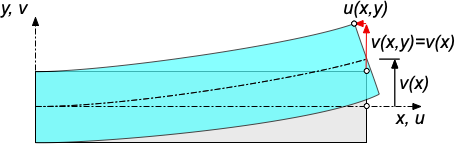
\includegraphics[scale=0.50]{beam.png}
		\caption{Deformation of the Bernoulli-Euler beam. Definition of coordinate axes and components of displacement.}
	\end{center}
	\label{Fig:1}
\end{figure}
This tool employs the Bernoulli-Euler beam theory.  This theory, also known as \emph{shear rigid beam theory}, is based on the kinematic assumption  that
\begin{quote}
   Any plane cross section perpendicular to the undeformed beam's axis remain plane and perpendicular to the axis throughout the deformation.
\end{quote}
This allows us to reduce the three-dimensional problem to a single unknown function, $v(x)$, known as \emph{deflection} of the beam.

\section{Kinematics}
Navier's assumption leads to
\begin{equation}
	u(x,y) = -y \,v'(x)
	\qquad
	v(x,y) = v(x)
	\label{Eq:1}
\end{equation}
This displacement field induces an axial strain of
\begin{equation}
	\varepsilon(x,y) = \frac{\partial u(x,y)}{\partial x} = -y\, v''(x) ~.
	\label{Eq:2}
\end{equation}
Equation~\eqref{Eq:2} states that a fiber parallel to the beam axis stretches in the bottom portion of the beam ($y<0$) and contracts if the fiber is located above the beam axis ($y>0$).  The beam axis itself  does not stretch.

\section{Constitutive relations}
For a slender beam, we can ignore stress components acting perpendicular to the beam's axis.  Thus, the constitutive relations can be simplified as the 1D-version of Hooke's law:
\begin{equation}
	\sigma(x,y) = E\,\varepsilon(x,y)
	\label{Eq:3}
\end{equation}
where $E$ is the modulus of elasticity.

The imposed state of deformation induces normal stress proportional to the strain field~\eqref{Eq:2} as
\begin{equation}
	\sigma(x,y) = -E y\,v''(x) ~.
	\label{Eq:4}
\end{equation}
This relation states that (i)~the stress varies linearly with the distance from the beam's axis, vanishing at the axis, and (ii)~the stress is proportional to the curvature of the beam.

\section{Stress resultants}
The beam sees two stress resultants: the internal moment, 
\begin{equation}
	M(x) = -\int_A y\sigma(x,y)\, dA
	\label{Eq:5}
\end{equation}
and the transverse shear force,
\begin{equation}
	V(x)  = -\int_A \tau_{xy}(x,y)\, dA
	\label{Eq:6}
\end{equation}
Substituting \eqref{Eq:4} into \eqref{Eq:5} yields
\begin{equation}
	M(x) = \int_A E y^2 \, v''(x) \, dA = E\,v''(x) \int_A y^2\,dA = EI\,v''(x)
	\label{Eq:7}
\end{equation}
where 
\begin{equation}
	I = \int_A y^2\,dA
	\label{Eq:7b}
\end{equation}
is the \emph{area moment of inertia} or, short, \emph{moment of inertia}.

Note that the modulus of elasticity, $E$, characterizes the material, the moment of inertia, $I$, characterized the shape of the cross section, and the second derivative of the deflection, $v''(x)$, characterizes the deformation (curvature) of the beam.

\section{Equilibrium}
Equilibrium is formulated in terms of shear forces, $V(x)$, and internal moments, $M(x)$.
Equilibrium of forces on an beam element of infinitesimal length, formulated in the $y$-direction, yields
\begin{equation}
	V'(x) = -w(x)
	\label{Eq:8}
\end{equation}
where $w(x)$ is the distributed lateral load per length.  $w(x)$ is defined positive if pointing against the (upward) positive $y$-axis.

Moment equilibrium around the out-of-plane axis on the same element yields
\begin{equation}
	M'(x) = V(x) ~.
	\label{Eq:9}
\end{equation}
A system for which equations~\eqref{Eq:8} and \eqref{Eq:9} are sufficient to determine the internal moment and shear functions is called \emph{statically determinate}. Otherwise, the system is called \emph{statically indeterminate}. Solving these equations for the latter requires consideration of the kinematic relation~\eqref{Eq:7} and respective boundary conditions.

Equations~\eqref{Eq:8} and \eqref{Eq:9} may be combined into one equation as
\begin{equation}
	M''(x) = V'(x)=-w(x)
	\label{Eq:10}
\end{equation}
Equation~\eqref{Eq:10} replaces both equilibrium equations \eqref{Eq:8} and \eqref{Eq:9}.

\section{Governing equation}
The governing equation is obtained by assuming the displacement function, $v(x)$, as the primary unknown and expressing $M(x)$ in \eqref{Eq:10} using \eqref{Eq:7} to obtain
\begin{equation}
	\left( EI(x)\,v''(x) \right)'' + w(x) = 0
	\label{Eq:11}
\end{equation}
This equation is known as the governing equation of the Bernoulli-Euler beam.

If the beam possesses a constant cross section and is made of one material, then $EI(x)=EI=const.$ and
\eqref{Eq:11} simplifies to
\begin{equation}
	EI\,v''''(x) + w(x) = 0
	\label{Eq:12}
\end{equation}
Equation~\eqref{Eq:12} is what is implemented in this program.

\section{Finding moment, shear force, and slope from the displacement function}
Solving \eqref{Eq:12} and applying suitable boundary conditions yields the displacement function, $v(x)$, for the beam.
The slope, $\theta(x)$, is obtained through differentiation as
\begin{equation}
	\theta(x) = v'(x) ~.
	\label{Eq:13}
\end{equation}
It is positive if the cross section rotates counter-clockwise during deformation.

The moment follows from \eqref{Eq:7} as
\begin{equation}
	M(x) = EI(x)\, v''(x) = EI(x)\, \theta'(x) ~.
	\label{Eq:14}
\end{equation}
The transverse shear force follows from~\eqref{Eq:10} as
\begin{equation}
	V(x) = M'(x) = \left( EI(x)\, v''(x) \right)'
	\label{Eq:15}
\end{equation}
or, for constant $EI$, simplifies to
\begin{equation}
	V(x) = EI\, v'''(x) ~.
	\label{Eq:16}
\end{equation}

\section{Examples}

\subsection{Single span beam with constant distributed force}

Both bending stiffness, $EI$, and distributed load, $w(x) = w_0$, are constant over the length of the beam.  Thus, \eqref{Eq:12} simplifies to
\begin{equation}
   v''''(x) =  -\frac{w_0}{EI}
   \label{A1}
\end{equation}
\begin{equation}
   v'''(x) =  -\frac{w_0\,x}{EI} + c_1
   \label{A2}
\end{equation}
\begin{equation}
   v''(x) =  -\frac{w_0\,x^2}{2 EI} + c_1\,x + c_2
   \label{A3}
\end{equation}
\begin{equation}
   \theta(x) = v'(x) =  -\frac{w_0\,x^3}{6 EI} + \frac{1}{2} \,c_1\,x^2 + c_2\,x + c_3
   \label{A4}
\end{equation}
\begin{equation}
   v(x) =  -\frac{w_0\,x^4}{24 EI} + \frac{1}{6} \,c_1\,x^3 + \frac{1}{2} \,c_2\,x^2+ c_3\,x + c_4
   \label{A5}
\end{equation}
\begin{equation}
   M(x) = EI \, v''(x) = -\frac{w_0\,x^2}{2} + EI\,c_1\,x + EI\,c_2
   \label{A6}
\end{equation}
\begin{equation}
   V(x) = M'(x) = EI \, v'''(x) = -w_0\,x + EI\,c_1
   \label{A7}
\end{equation}
Pinned on both ends yields the boundary conditions
\begin{equation}
%   v(0) = 0 ~,~~~
%   M(0) = 0 ~,~~~
%   v(\ell) = 0 ~,~~~
%   M(\ell) = 0 ~.
%  
   \left\{ 
   \begin{array}{c}
   v(0) \\
   M(0) \\
   v(\ell) \\
   M(\ell) 
   \end{array}
   \right\}
   =
   \left\{ 
   \begin{array}{c}
    0 \\
    0 \\
    0 \\
    0 
   \end{array}
   \right\}
   \label{A8}
\end{equation}
\begin{equation}
   \left[ 
   \begin{array}{cccc}
    0 & 0 & 0 & 1 \\
    0 & EI & 0 & 0 \\
    \ell^3/6 & \ell^2/2 & \ell & 1 \\
    EI\,\ell & EI & 0 & 0 
   \end{array}
   \right]
   \left\{ 
   \begin{array}{c}
    c_1 \\
    c_2 \\
    c_3 \\
    c_4 
   \end{array}
   \right\}
   =
   \left\{ 
   \begin{array}{c}
    0 \\
    0 \\
    \DS\frac{w_0 \ell^4}{24\, EI} \\[2ex]
    \DS\frac{w_0 \ell^2}{2}
   \end{array}
   \right\}
   \label{A9}
\end{equation}
\begin{equation}
   \left\{ 
   \begin{array}{c}
    c_1 \\
    c_2 \\
    c_3 \\
    c_4 
   \end{array}
   \right\}
   =
   \left\{ 
   \begin{array}{c}
    \DS\frac{w_0 \ell}{2\, EI} \\[2ex]
    0 \\
    \DS-\frac{w_0 \ell^3}{24\, EI} \\[2ex]
    0
   \end{array}
   \right\}
   \label{A10}
\end{equation}
\begin{equation}
   v(x) 
   % =  -\frac{w_0\,x^4}{24 EI} + \frac{w_0 \ell}{12\, EI}\,x^3  -\frac{w_0 \ell^3}{24\, EI}\,x 
   =  \frac{w_0\,\ell^4}{24 EI} \, \frac{x}{\ell} \left( 1 -\frac{x}{\ell}  \right)\left( \frac{x^2}{\ell^2} -\frac{x}{\ell}  - 1 \right)
   \label{A11}
\end{equation}
\begin{equation}
   M(x) = EI\,v''(x) = \frac{w_0\,\ell^2}{2} \,\frac{x}{\ell} \left( 1 -\frac{x}{\ell}  \right)
   \label{A12}
\end{equation}
\begin{equation}
   V(x) = M'(x) = EI\,v'''(x) = \frac{w_0\,\ell}{2} \left( 1 - 2\frac{x}{\ell}  \right)
   \label{A13}
\end{equation}
Shear vanishes at $x=\ell$ and, thus,
\begin{equation}
   \max M = M(\ell/2) = \frac{w_0\,\ell^2}{8} 
   \label{A14}
\end{equation}
By symmetry, rotation vanishes at $x=\ell$ and, thus,
\begin{equation}
   \max |v| = -\min v = -v(\ell/2) = \frac{5 w_0\,\ell^4}{384 EI}
   \label{A15}
\end{equation}

\subsection{Single span beam with a single concentrated force}

\begin{eqnarray}
   v_1''''(x) &=&  0 \\
   v_1'''(x) &=&   c_1 \\
   v_1''(x) &=&   c_1\,x + c_2  \\
   \theta_1(x) = v_1'(x) &=&  \frac{1}{2} \,c_1\,x^2 + c_2\,x + c_3 \\
   v_1(x) &=&  \frac{1}{6} \,c_1\,x^3 + \frac{1}{2} \,c_2\,x^2+ c_3\,x + c_4 \\
   M_1(x) = EI \, v_1''(x) &=&  EI\,c_1\,x + EI\,c_2 \\
   V_1(x) = M_1'(x) = EI \, v_1'''(x) &=& EI\,c_1
   \label{B1}
\end{eqnarray}
\begin{eqnarray}
   v_2''''(x) &=&  0 \\
   v_2'''(x) &=&   d_1 \\
   v_2''(x) &=&   d_1\,x + d_2  \\
   \theta_2(x) = v_2'(x) &=&   \frac{1}{2} \,d_1\,x^2 + d_2\,x + d_3 \\
   v_2(x) &=&   \frac{1}{6} \,d_1\,x^3 + \frac{1}{2} \,d_2\,x^2+ d_3\,x + d_4 \\
   M_2(x) = EI \, v_2''(x) &=&  EI\,d_1\,x + EI\,d_2 \\
   V_2(x) = M_2'(x) = EI \, v_2'''(x) &=&  EI\,d_1
   \label{B2}
\end{eqnarray}
Boundary conditions
\begin{equation}
   \left\{ 
   \begin{array}{c}
   v(0) = v_1(0) \\
   M(0) = M_1(0) \\
   v(\ell) = v_2(\ell) \\
   M(\ell) = M_2(\ell)
   \end{array}
   \right\}
   =
   \left\{ 
   \begin{array}{c}
    0 \\
    0 \\
    0 \\
    0 
   \end{array}
   \right\}
   \label{B3}
\end{equation}
Continuity conditions:
\begin{equation}
   v_1(a) = v_2(a)
   \qquad\hbox{and}\qquad
   \theta_1(a) = \theta_2(a)
   \label{B4}
\end{equation}
Equilibrium of forces for the interval $[a-\epsilon,a+\epsilon]$:
\begin{equation}
   \lim_{\epsilon\to 0} \left[ V(a-\epsilon) - P - V(a+\epsilon)  \right] = 0
   \qquad\Rightarrow\quad
   V_1(a) - V_2(a) = P
   \label{B5}
\end{equation}
Moment equilibrium for the interval $[a-\epsilon,a+\epsilon]$:
\begin{equation}
   \lim_{\epsilon\to 0} \left[ M(a-\epsilon) + \epsilon V(a-\epsilon) - M(a+\epsilon) + \epsilon V(a+\epsilon) \right] = 0
   \quad\Rightarrow\quad
   M_1(a) = M_2(a)
   \label{B6}
\end{equation}
\begin{equation}
   \left[ 
   \begin{array}{cccccccc}
    0 & 0 & 0 & 1 & 0 & 0 & 0 & 0 \\[2ex]
    0 & EI & 0 & 0 & 0 & 0 & 0 & 0 \\[2ex]
    0 & 0 & 0 & 0 & \ell^3/6 & \ell^2/2 & \ell & 1 \\[2ex]
    0 & 0 & 0 & 0 & EI\,\ell & EI & 0 & 0 \\[2ex]
    a^3/6 & a^2/2 & a & 1 & -a^3/6 & -a^2/2 & -a & -1 \\[2ex]
    a^2/2 & a & 1 & 0 & -a^2/2 & -a & -1 & 0 \\[2ex]
    EI \,a & EI & 0 & 0 & -EI\,a & -EI & 0 & 0 \\[2ex]
    EI & 0 & 0 & 0 & -EI & 0 & 0 & 0 
   \end{array}
   \right]
   \left\{ 
   \begin{array}{c}
    c_1 \\[1.5ex]
    c_2 \\[1.5ex]
    c_3 \\[1.5ex]
    c_4 \\[1.5ex]
    d_1 \\[1.5ex]
    d_2 \\[1.5ex]
    d_3 \\[1.5ex]
    d_4
   \end{array}
   \right\}
   =
   \left\{ 
   \begin{array}{c}
    0 \\[1.5ex]
    0 \\[1.5ex]
    0 \\[1.5ex]
    0 \\[1.5ex]
    0 \\[1.5ex]
    0 \\[1.5ex]
    0 \\[1.5ex]
    P 
   \end{array}
   \right\}
   \label{B7}
\end{equation}
Using $\alpha=a/\ell$, the integration constants are obtained as
\begin{equation}
   \left\{ 
    c_1 \,,~
    c_2 \,,~
    c_3 \,,~
    c_4 
   \right\}
   =
   \left\{
   	\frac{ (1-\alpha)  P}{{EI}},~
	0,~
	-\frac{ \alpha  \left(\alpha ^2-3 \alpha +2\right) P \ell^2 }{6 \,{EI}},~
   	0
   \right\}
   \label{B8}
\end{equation}
and
\begin{equation}
   \left\{ 
    d_1 \,,~
    d_2 \,,~
    d_3 \,,~
    d_4
   \right\}
   =
   \left\{
	\frac{ -\alpha  P}{2 {EI}},~
	\frac{\alpha  P \ell }{{EI}},~
	-\frac{ \alpha  \left(2+\alpha^2\right) P \ell^2 }{6 \,{EI}},~
	\frac{\alpha^3  P \ell^3}{6 \,{EI}}
   \right\}
   \label{B9}
\end{equation}
\begin{equation}
   \label{B10}
\end{equation}
\begin{equation}
   \label{B11}
\end{equation}
\begin{equation}
   \label{B12}
\end{equation}
\begin{equation}
   \label{B13}
\end{equation}
\begin{equation}
   \label{B14}
\end{equation}
\begin{equation}
   \label{B15}
\end{equation}
\begin{equation}
   \label{B16}
\end{equation}
\begin{equation}
   \label{B17}
\end{equation}
\begin{equation}
   \label{B18}
\end{equation}

\subsection{Single span beam with a concentrated force and distributed load using the stiffness method}

\begin{equation}
   \label{C1}
\end{equation}
\begin{equation}
   \label{C2}
\end{equation}
\begin{equation}
   \label{C3}
\end{equation}
\begin{equation}
   \label{C4}
\end{equation}
\begin{equation}
   \label{C5}
\end{equation}
\begin{equation}
   \label{C6}
\end{equation}
\begin{equation}
   \label{C7}
\end{equation}
\begin{equation}
   \label{C8}
\end{equation}
\begin{equation}
   \label{C9}
\end{equation}
\begin{equation}
   \label{C10}
\end{equation}

\end{document}  